\documentclass[12pt,fleqn]{article}\usepackage{../../common}
\begin{document}
Iki Imaj Kullanarak 3 Boyutta Tekrar Olusturmak (3D Reconstruction from Two Images)

\begin{minted}[fontsize=\footnotesize]{python}
from mpl_toolkits.mplot3d import axes3d
import scipy.linalg as lin
import cv2

dir = "/home/burak/Documents/Dropbox/Public/data/pcv_data"
img1 = cv2.imread(dir + "/alcatraz1.jpg")
img2 = cv2.imread(dir + "/alcatraz2.jpg")

detector = cv2.ORB_create( nfeatures = 10000 )

def detect_features(frame):
    keypoints, descrs = detector.detectAndCompute(frame, None)
    if descrs is None: descrs = []
    return keypoints, descrs

FLANN_INDEX_LSH    = 6
flann_params= dict(algorithm = FLANN_INDEX_LSH,
                   table_number = 6, # 12
                   key_size = 12,     # 20
                   multi_probe_level = 1) #2


kp1, des1 = detect_features(img1)
kp2, des2 = detect_features(img2)

matcher = cv2.FlannBasedMatcher(flann_params, {})
matches = matcher.knnMatch(des1, des2, k = 2)

matches = [m[0] for m in matches \
           if len(m) == 2 and m[0].distance < m[1].distance * 0.75]

print 'matches', len(matches)

pts1 = []; pts2 = []

for i in range(len(matches)):
    pt_a = kp1[matches[i].queryIdx].pt
    pt_b = kp2[matches[i].trainIdx].pt
    pt_a = np.array(pt_a).astype(int)
    pt_b = np.array(pt_b).astype(int)
    if np.sqrt(np.dot(pt_b-pt_a,pt_b-pt_a)) < 200:
        pts1.append(pt_a)
        pts2.append(pt_b)
        cv2.line(img1, tuple(pt_a), tuple(pt_b), (255, 0, 0), 5)
        cv2.circle(img1,tuple(pt_b), 5, (0,0,255), -1)

h,w,d = img1.shape
tmp = cv2.resize(img1, (int(w/4),int(h/4)))
cv2.imwrite('vision_20recons_01.jpg',tmp)

for pt in pts2: cv2.circle(img2,tuple(pt),5,(0,0,255),-1)
tmp = cv2.resize(img2, (int(w/4),int(h/4)))
cv2.imwrite('vision_20recons_02.jpg',tmp)
\end{minted}

\begin{verbatim}
matches 1277
Out[1]: 
True
\end{verbatim}

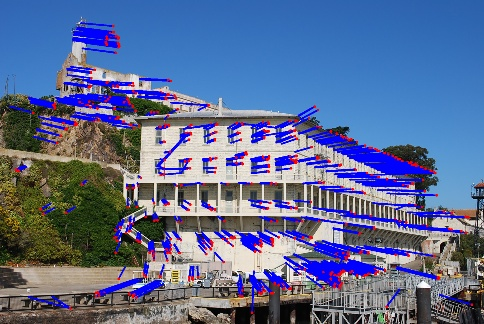
\includegraphics[width=30em]{vision_20recons_01.jpg}

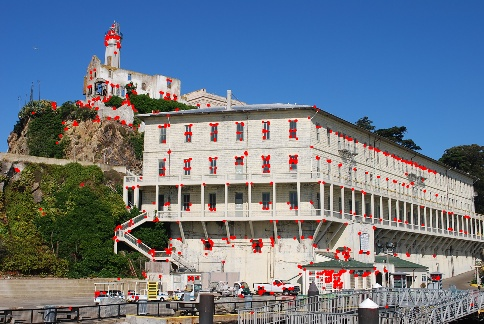
\includegraphics[width=30em]{vision_20recons_02.jpg}


\begin{minted}[fontsize=\footnotesize]{python}
# kamera matrisi biliniyor
K = np.array([[2394,0,932],[0,2398,628],[0,0,1]])

h,w,dum = img1.shape
pts1[:,1] = h-pts1[:,1]
pts2[:,1] = h-pts2[:,1]

F, mask = cv2.findFundamentalMat(pts1,pts2)

E = K.T.dot(F).dot(K)

R1,R2,t = cv2.decomposeEssentialMat(E)
\end{minted}


\begin{minted}[fontsize=\footnotesize]{python}
def triangulate_point(u1, u2, P1, P2):
  A = [[u1[0]*P1[2,0]-P1[0,0],u1[0]*P1[2,1]-P1[0,1],u1[0]*P1[2,2]-P1[0,2]],
       [u1[1]*P1[2,0]-P1[1,0],u1[1]*P1[2,1]-P1[1,1],u1[1]*P1[2,2]-P1[1,2]],
       [u2[0]*P2[2,0]-P2[0,0],u2[0]*P2[2,1]-P2[0,1],u2[0]*P2[2,2]-P2[0,2]],
       [u2[1]*P2[2,0]-P2[1,0],u2[1]*P2[2,1]-P2[1,1],u2[1]*P2[2,2]-P2[1,2]]]
  B = [[-(u1[0]*P1[2,3]-P1[0,3])],
       [-(u1[1]*P1[2,3]-P1[1,3])],
       [-(u2[0]*P2[2,3]-P2[0,3])],
       [-(u2[1]*P2[2,3]-P2[1,3])]]
  A = np.array(A)
  B = np.array(B)
  X = lin.lstsq(A,B)[0].T[0]
  res = np.array([X[0],X[1],X[2],1])
  return res

def triangulate(x1, x2, P1, P2):
  X = [triangulate_point(x1[i, :], x2[i, :], P1, P2) for i in range(len(x1))]
  return np.array(X).T


P1 = np.eye(4)
P2 = np.array([[ 0.878, -0.01 ,  0.479, -1.995],
              [ 0.01 ,  1.   ,  0.002, -0.226],
              [-0.479,  0.002,  0.878,  0.615],
              [ 0.   ,  0.   ,  0.   ,  1.   ]])
# Homogeneous arrays
a3xN = np.array([[ 0.091,  0.167,  0.231,  0.083,  0.154],
                 [ 0.364,  0.333,  0.308,  0.333,  0.308],
                 [ 1.   ,  1.   ,  1.   ,  1.   ,  1.   ]])
b3xN = np.array([[ 0.42 ,  0.537,  0.645,  0.431,  0.538],
                 [ 0.389,  0.375,  0.362,  0.357,  0.345],
                 [ 1.   ,  1.   ,  1.   ,  1.   ,  1.   ]])
X = triangulate_point( a3xN.T[0], b3xN.T[0], P1, P2 )
X /= X[3]
x1 = np.dot(P1[:3],X)
x2 = np.dot(P2[:3],X)
x1 /= x1[2]
x2 /= x2[2]
 
print 'X', X
print 'x', x1
print 'x2', x2
\end{minted}

\begin{verbatim}
X [  1.00277411   4.01217675  11.01977032   1.        ]
x [ 0.09099773  0.36408896  1.        ]
x2 [ 0.4200205   0.38890029  1.        ]
\end{verbatim}


\begin{minted}[fontsize=\footnotesize]{python}
for i,P in enumerate(((R1,t),(R1,-t),(R2,t),(R2,-t))):

    P1 = K.dot(np.hstack(P))       # Projection matrix of second cam is ready
    print 'P', P1

    P00 = np.float64([ [1,0,0,0],
                       [0,1,0,0],
                       [0,0,1,0]   ]) # Projection matrix of first cam at origin
    P0 = K.dot(P00) 

    X = triangulate(pts1, pts2, P0, P1)

    fig = plt.figure()
    ax = fig.gca(projection='3d')    
    ax.plot(X[0], X[2], X[1], 'r.')
    ax.view_init(elev=23., azim=-67)
    plt.savefig('thd_03_%d.png' % i)
\end{minted}




















\end{document}




















